\documentclass{beamer}
\usetheme{Pittsburgh}
\usecolortheme{whale}
\usepackage[T1]{fontenc}
%\usepackage[utf8]{inputenc}
\usepackage[frenchb]{babel}
\usepackage{listings}
\usepackage{amsmath}
\usepackage{hyperref}

%Gummi|065|=)
\beamertemplatenavigationsymbolsempty
\title{\textbf{Sécurité RDP : Intecteption d'authentification sur NLA avec CredSSPy}}
\author{Geoffrey Bertoli -- @yofbalibump (Synacktiv)\\
		Thomas Bourguenolle (EY)
		}
\titlegraphic{
\includegraphics[width=4cm]{Logo_sstic.png}}
\date{}
\logo{%
	
\includegraphics[width=2cm,height=2cm,keepaspectratio]{synacktiv_logo.jpeg}~%
	 \hspace{93mm}
	
\includegraphics[width=1cm,height=1cm,keepaspectratio]{EY-logo-.png}%
}
\begin{document}
	
	\setbeamertemplate{footnote}{
		\footnotesize
		\hspace*{1.7cm}%
		\raisebox{3ex}{\insertfootnotemark}
		\parbox[b][0cm]{8cm}{
			\insertfootnotetext%
		}%
	} 
\begin{frame}
\titlepage
\end{frame}

\section{Introduction}

\begin{frame}
\frametitle{Table des matières}
\tableofcontents[currentsection]
\end{frame}



%slide 1
\begin{frame}{Mode d'authentification pour RDP}
	\begin{columns}
	\column {\textwidth}
		\begin{itemize}
		\item Les serveurs RDP supportent actuellement 3 modes d’authentification
		distincts pour l’établissement d’une connexion :
		\begin{itemize}
		\item \textbf{RDP Standard Security} :  Les échanges entre le client et le
		serveur sont chiffrés à l’aide d’une clé symétrique. Cette clé est
		négociée à partir d’un échange RSA établi avec une paire de clés
		fixe spécifiée dans la documentation Microsoft.
		\item \textbf{RDP Enhanced sécurity TLS} (Depuis RDP 5.2) :  Les échanges
		entre le client et le serveur sont chiffrés à l’aide d’une clé symétrique
		négociée dans un canal TLS.
		\item \textbf{RDP Enhanced security NLA} (Depuis RDP 6.0) Mode d’au-
		thentification par défaut depuis Windows Server 2012R2. Basé sur CredSSP, les échanges entre
		le client et le serveur sont chiffrés à l'aide d’une clé symétrique
		négociée dans un canal TLS après « authentification mutuelle » des
		deux acteurs (via Kerberos ou NTLMSSP)
		\end{itemize}
		\end{itemize}
	\end{columns}
   \end{frame}

%slide 2
\begin{frame}{Mode d'authentification  pour RDP}
	\begin{columns}[T]
	\column {.6\textwidth}
		\begin{itemize}
		\item Authentication pré-NLA
		\begin{figure}
		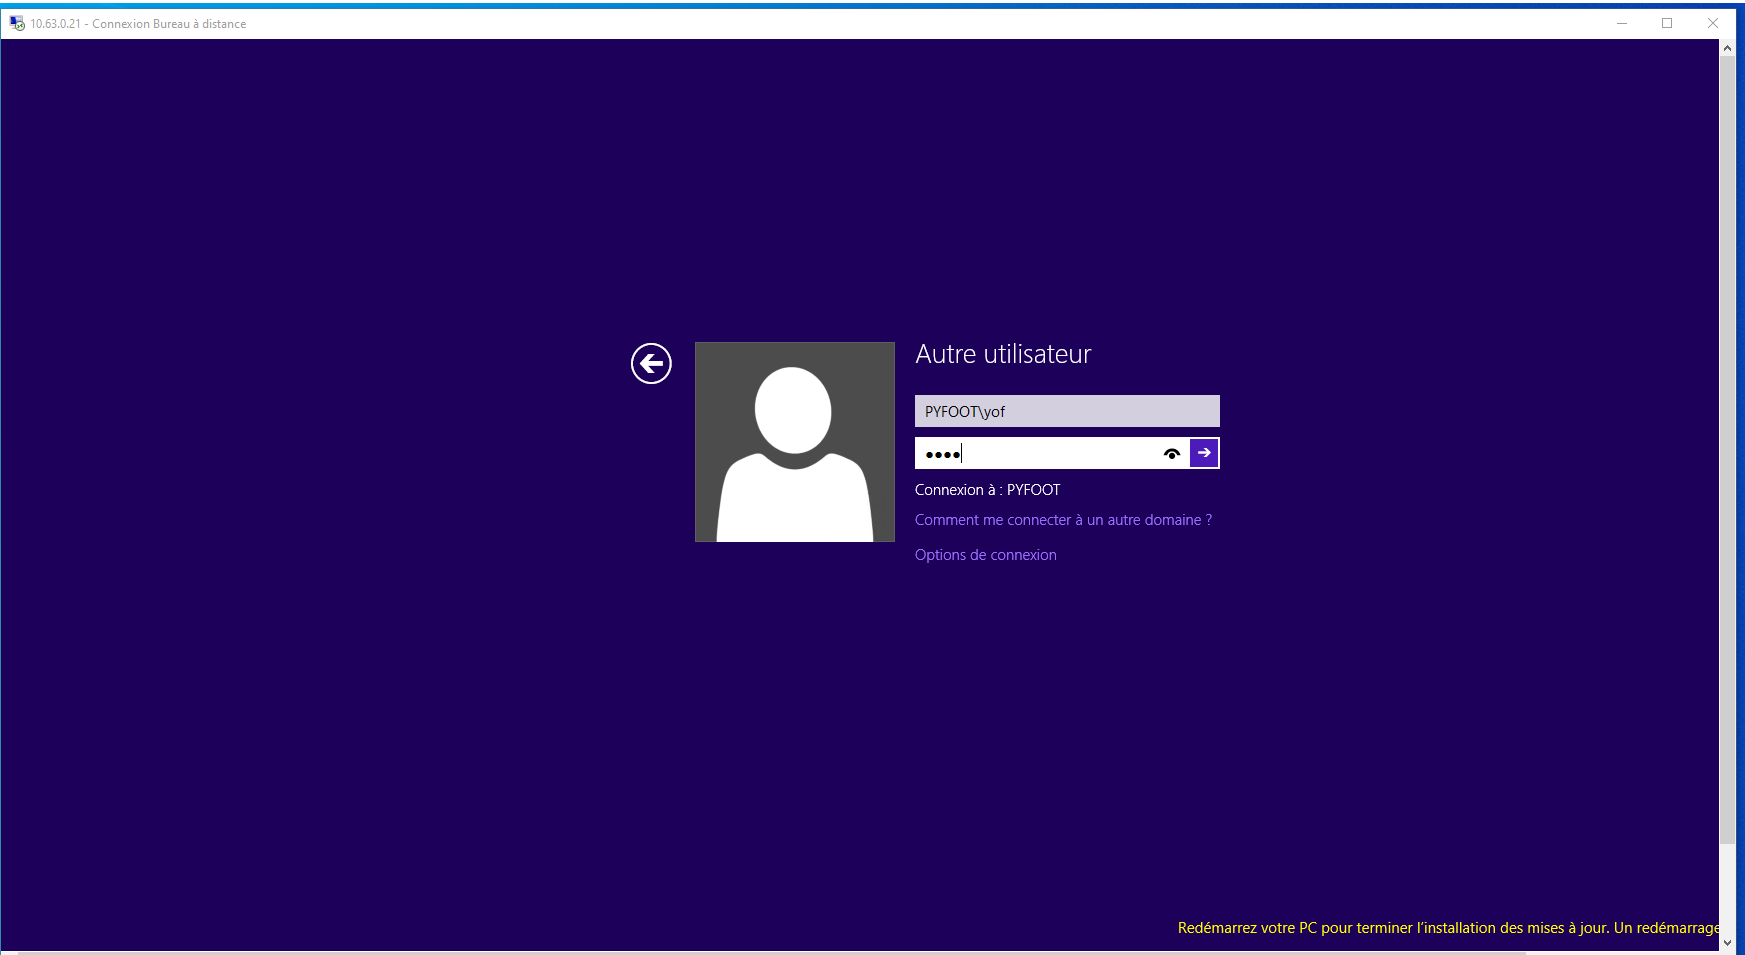
\includegraphics[scale=0.10]{No_NLA.png}
	\end{figure}
		\end{itemize}
	\column {.7\textwidth}
		\begin{itemize}
		\item  Authentification avec NLA
		\begin{figure}
		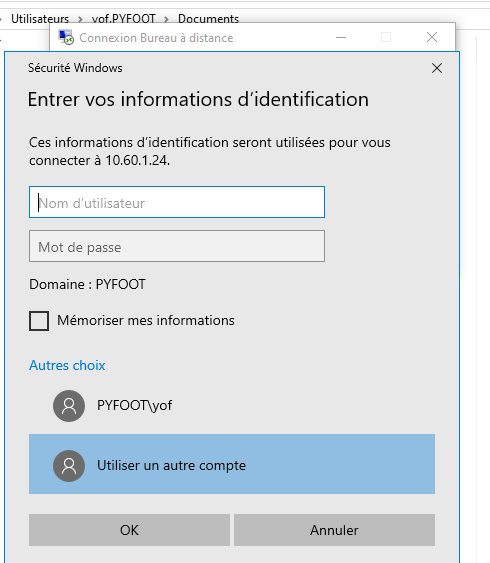
\includegraphics[width=100pt,height=120pt]{NLA.png}
		\end{figure}
		\end{itemize}
	\end{columns}
\end{frame}


%slide 3
\begin{frame}[fragile]{Rapide état de l'art}
	\begin{itemize}
	\item Plusieurs outils permettent actuellement la mise en place d'attaques de type Man-In-The-Middle sur RDP
	\item SETH, PyRDP ou encore rdpy nécessitent de forcer le client à utiliser un mode d'authentification moins sécurisé
	\item Un article présenté à SSTIC 2012\footnotemark, indique cependant la possibilité d'une telle attaque dans le cas ou une machine du domaine serait compromise
	\end{itemize}
\footnotetext[1]{Sécurité de RDP : \url{https://www.sstic.org/2012/presentation/securite\_rdp/}}
\end{frame}

\section{CredSSP - Description du protocole}


\begin{frame}
	\frametitle{Table des matières}
	\tableofcontents[currentsection]
\end{frame}


%slide 3
\begin{frame}{CredSSP}
Le protocole Credential Security Support Provider (CredSSP) permet à une application de transmettre de manière sécurisé des authentifiants à une application cible
\newline

Le protocole utilise d'abord un canal TLS non approuvé. Ensuite  à l'aide du protocole SPNEGO  une authentification « mutuelle » du serveur et du client est effectuée
Les authentifiants (ici ceux de l'utilisateur de la session RDP) sont ensuite envoyés à l'intérieur de ce canal TLS
\newline
\begin{center}
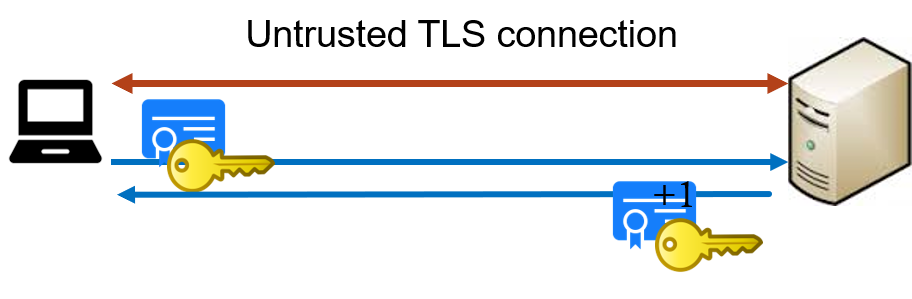
\includegraphics[width=0.8\textwidth,height=0.3\textheight]{credssp.png}
\end{center}
\end{frame}

%slide 4
\begin{frame}{CredSSP - Description du protocole}
\begin{figure}
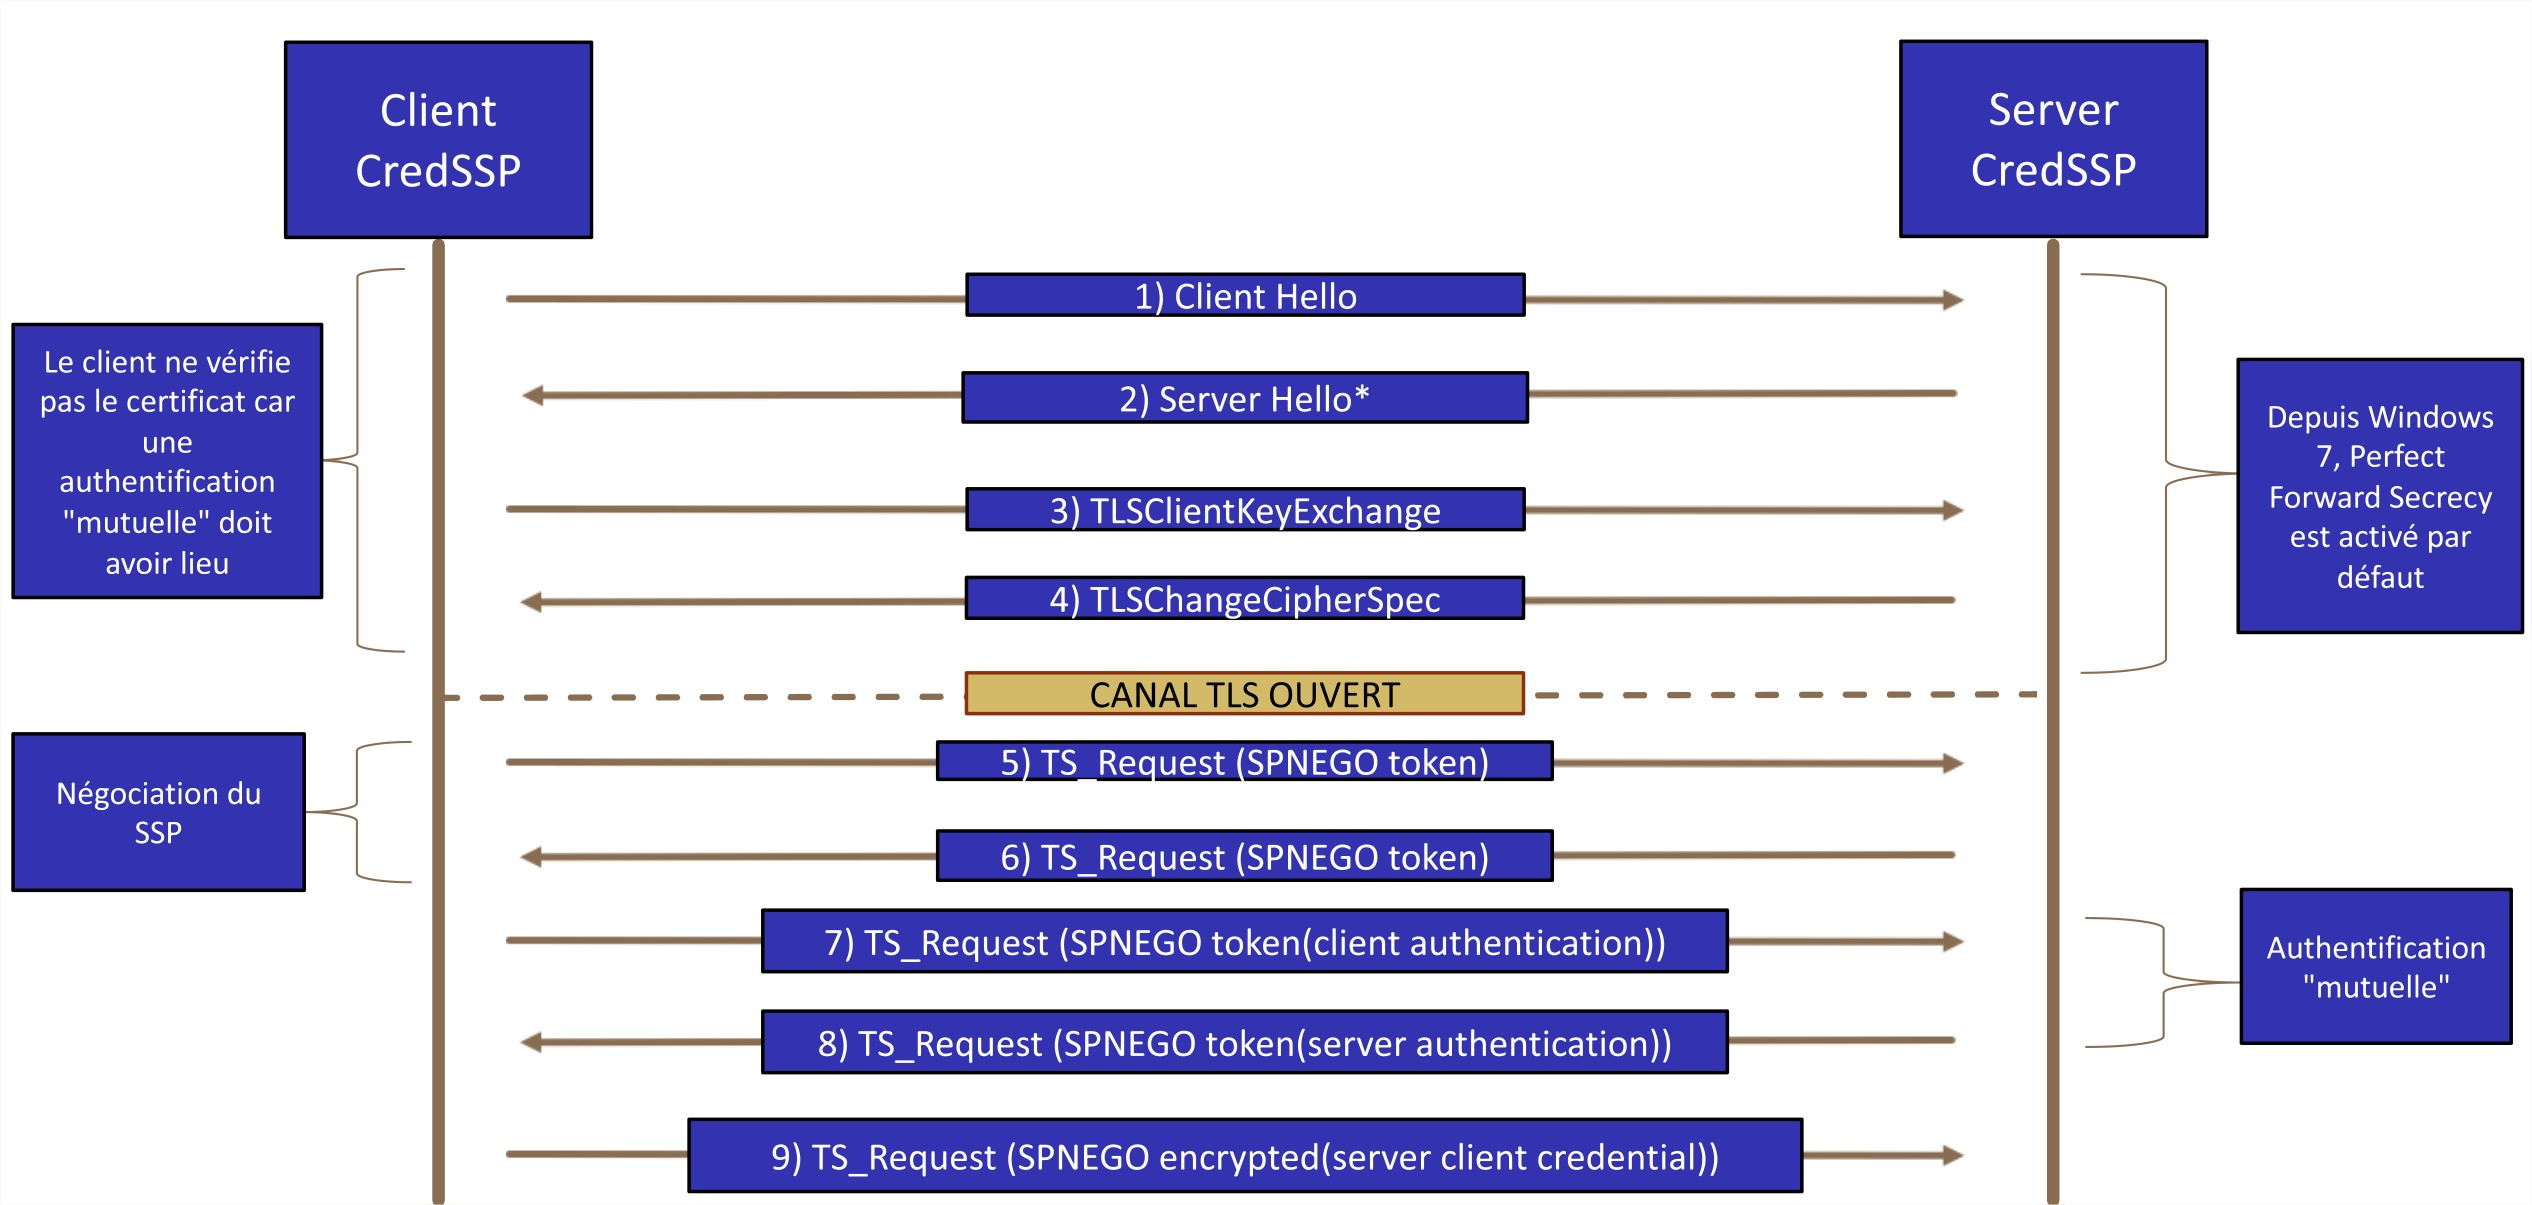
\includegraphics[scale=0.16]{graph.jpg}
\end{figure}
\end{frame}


%slide 6
\begin{frame}[fragile]{CredSSP - TS\_Request}
	\begin{itemize}
		\item La TSRequest est la structure principale d'un paquet CredSSP. Elle encapsule le jeton SPNEGO ainsi que les potentiels messages Kerberos ou NTLM échangés entre le serveur et le client
		\item TSRequest structure :
		\begin{columns}[T]
			\column {.6\textwidth}
			\begin{lstlisting}[frame=single,basicstyle=\tiny]
TSRequest :== SEQUENCE {		
	
	Version     [0] INTEGER,
	
	negoToken   [1] NegoData OPTIONNAL,
	
	authInfo    [2] OCTET STRING OPTIONNAL,
	
	pubKeyAuth  [3] OCTET STRING OPTIONNAL,
	
	errorCode   [4] OCTET STRING OPTIONNAL,
	
	clientNonce [5] OCTET STRING OPTIONNAL
	
	}
			\end{lstlisting}
			\column {.4\textwidth}
			\begin{itemize}
				\footnotesize \item La présentation traitera la version 6 de CredSSP
				\footnotesize \item Depuis la vulnérabilité CVE-2018-0886, le client Microsoft refuse les connexions à un serveur utilisant la version 5 ou inférieure (par défaut)
			\end{itemize}
		\end{columns}
	\end{itemize}
\end{frame}

%slide 5
\begin{frame}{CredSSP - Description du protocol}
	\begin{itemize}
	\item Pendant l'étape 5 et 6, le serveur et le client négocient quel SSP utiliser. Il est possible d'utiliser NLTMSSP ou Kerberos
	\newline
	
	\item NTLMSSP sera choisi si :
		\begin{itemize}
		\item Le client n'appartient pas à un domaine \textbf{OU}
		\item Le client utilise l'adresse IP pour se connecter au serveur 
		\newline 
		
		\end{itemize}
	\item Kerberos sera choisi si :
		\begin{itemize}
		\item Le client et le domaine appartiennent au même domaine \textbf{ET}
		\item Le client utilise le FQDN du serveur pour la connexion
		\end{itemize}
	\end{itemize}
\end{frame}


\section{CredSSP - NTLMSSP}

\begin{frame}
	\frametitle{Table des matières}
	\tableofcontents[currentsection]
\end{frame}

%slide 7
\begin{frame}[fragile]{CredSSP - NTLMSSP Etape 5}
	 \begin{columns}[T]
	 \column{0.7\textwidth}
	 	\begin{itemize}
	 	\item Le client envoie un message indiquant qu'il souhaite utiliser NTLM comme SSP
	 	\end{itemize}
	 \begin{lstlisting}[frame=single,basicstyle=\tiny]
TSRequest {
	Version:     6,
	negoToken:   NegoData-> NTLMSS NEGOTIATE\_MESSAGE
	}
	\end{lstlisting}
	 \column {0.3\textwidth}
	 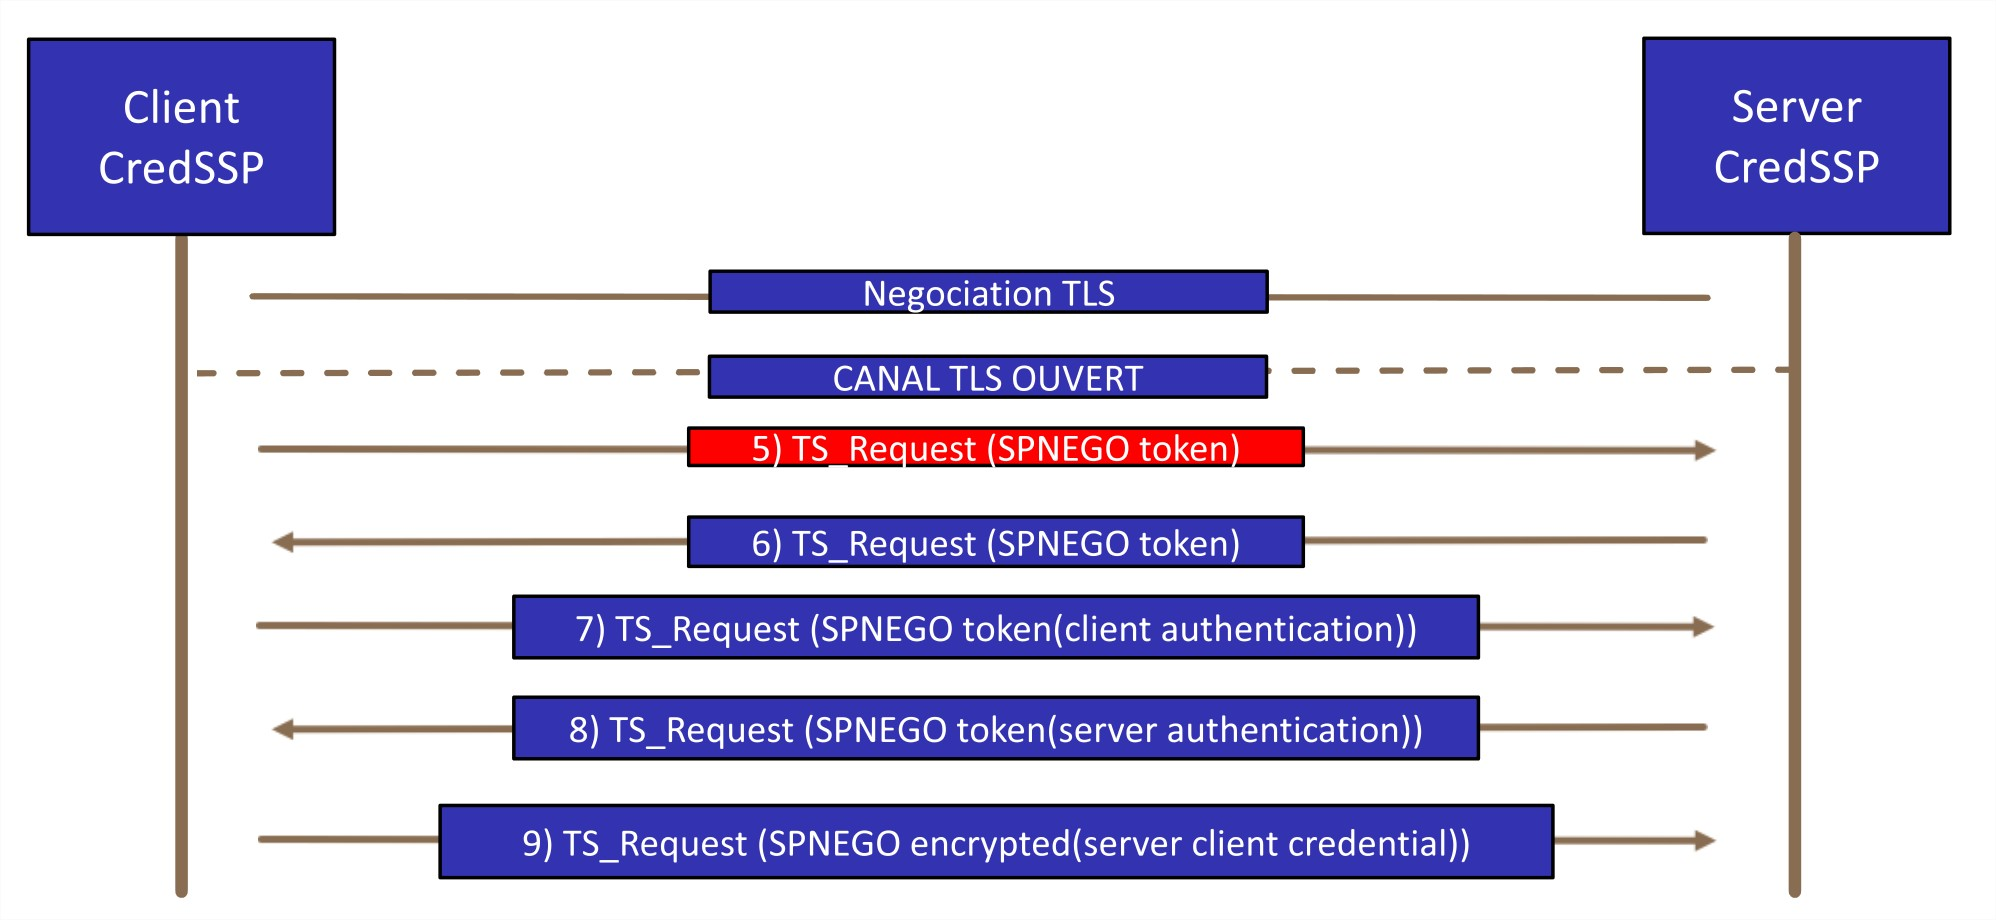
\includegraphics[scale=0.07]{step5.jpg}
	 \end{columns}
	 
	 \begin{itemize}
	 	\item Le NTLMSSP NEGOTIATE\_MESSAGE contient les informations sur la version de NTLMSSP supportée ainsi que les flags à utiliser
	 	\end{itemize}
\end{frame}

%slide 8
\begin{frame}[fragile]{CredSSP - NTLMSSP Etape 6}
	 \begin{columns}[T]
	 \column{0.7\textwidth}
	 	\begin{itemize}
	 	\item Le serveur renvoie alors un challenge NTLM
	 	\end{itemize}
	 \begin{lstlisting}[frame=single,basicstyle=\tiny]
TSRequest {
	Version:     6,
	negoToken:   NegoData-> NTLMSSP CHALLENGE\_MESSAGE
	}
	\end{lstlisting}
	 \column {0.3\textwidth}
	 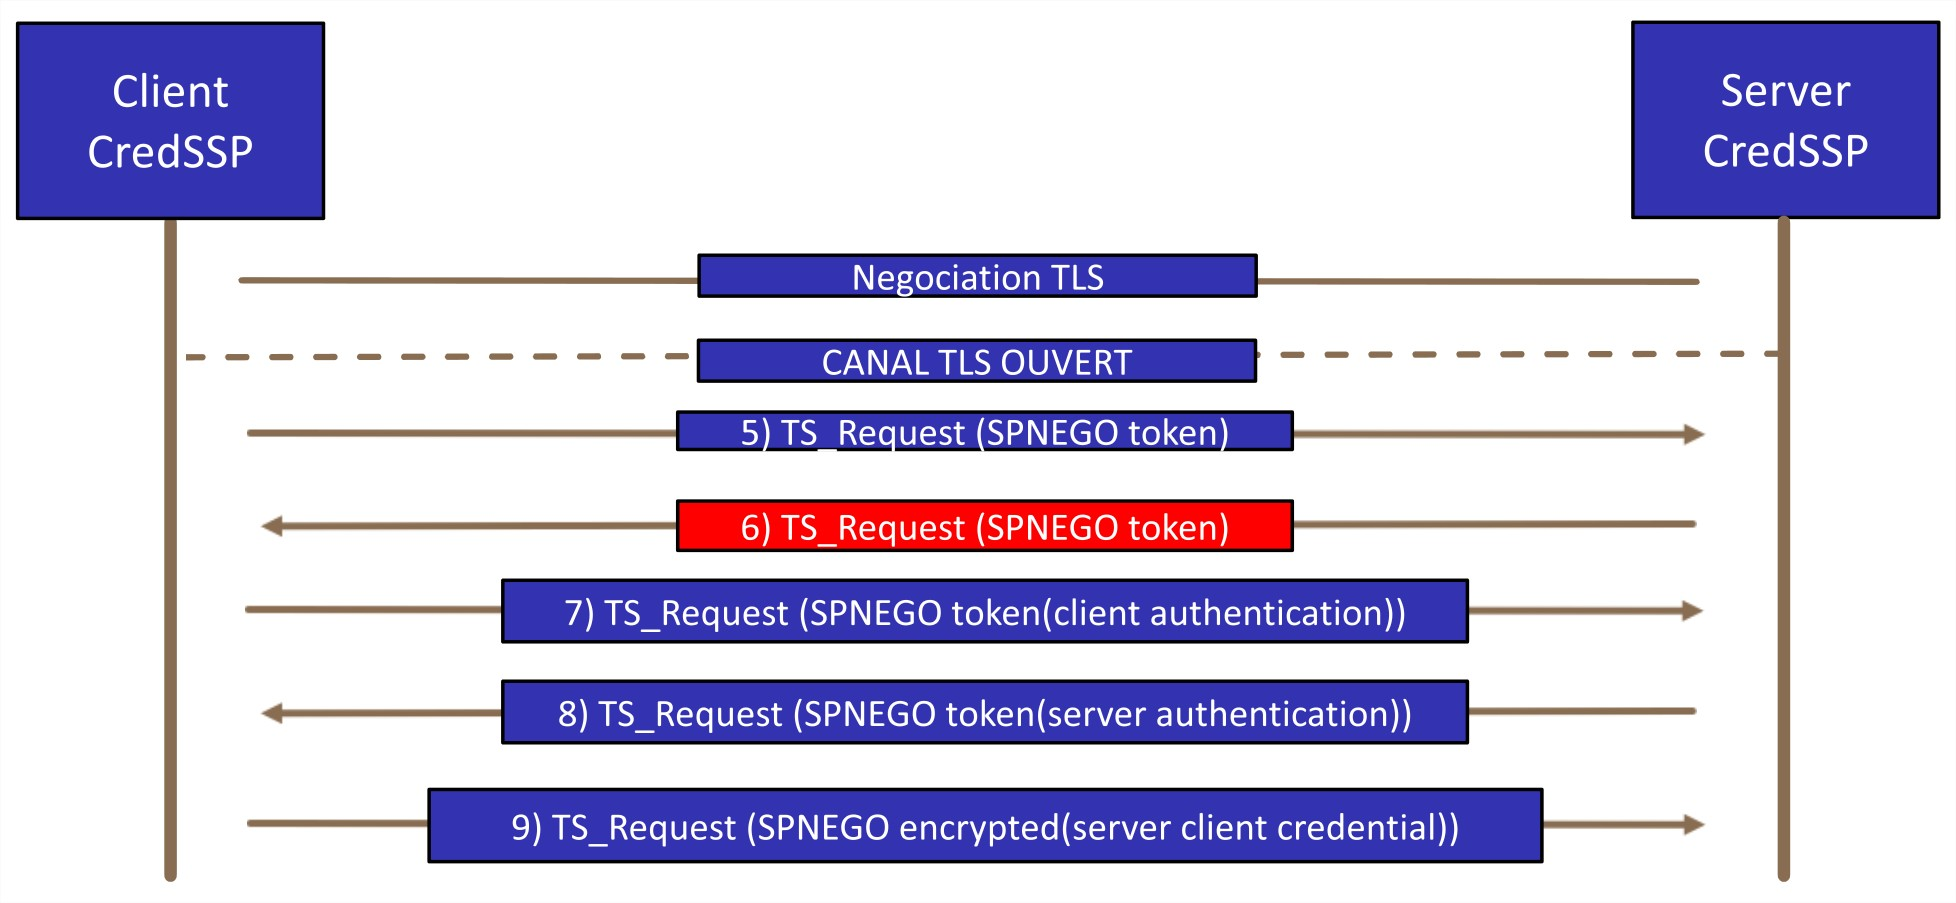
\includegraphics[scale=0.07]{step6.jpg}
	 \end{columns}
	 
	 \begin{itemize}
	 	\item NTLMSSP CHALLENGE\_MESSAGE est le challenge NTLM contenant :
	 		\begin{itemize}
	 		\item NTLMChallenge
	 		\item Server name
	 		\item Domain name
	 		\end{itemize}
	 	\end{itemize}
\end{frame}

%slide 9
\begin{frame}[fragile]{CredSSP - NTLMSSP Etape 7}
	 \begin{columns}[T]
	 \column{0.7\textwidth}
	 	\begin{itemize}
	 	\item Le client répond au challenge et demande une vérification de l'intégrité de l'échange TLS
	 	\end{itemize}
	 \begin{lstlisting}[frame=single,basicstyle=\tiny]
TSRequest {
	Version:     6,
	negoToken:   NegoData-> NTLMSSP AUTHENTICATE\_MESSAGE,
	pubKeyAuth: Signature + encryptedpubKey,
	clientNonce: Octet String
	}
	\end{lstlisting}
	 \column {0.3\textwidth}
	 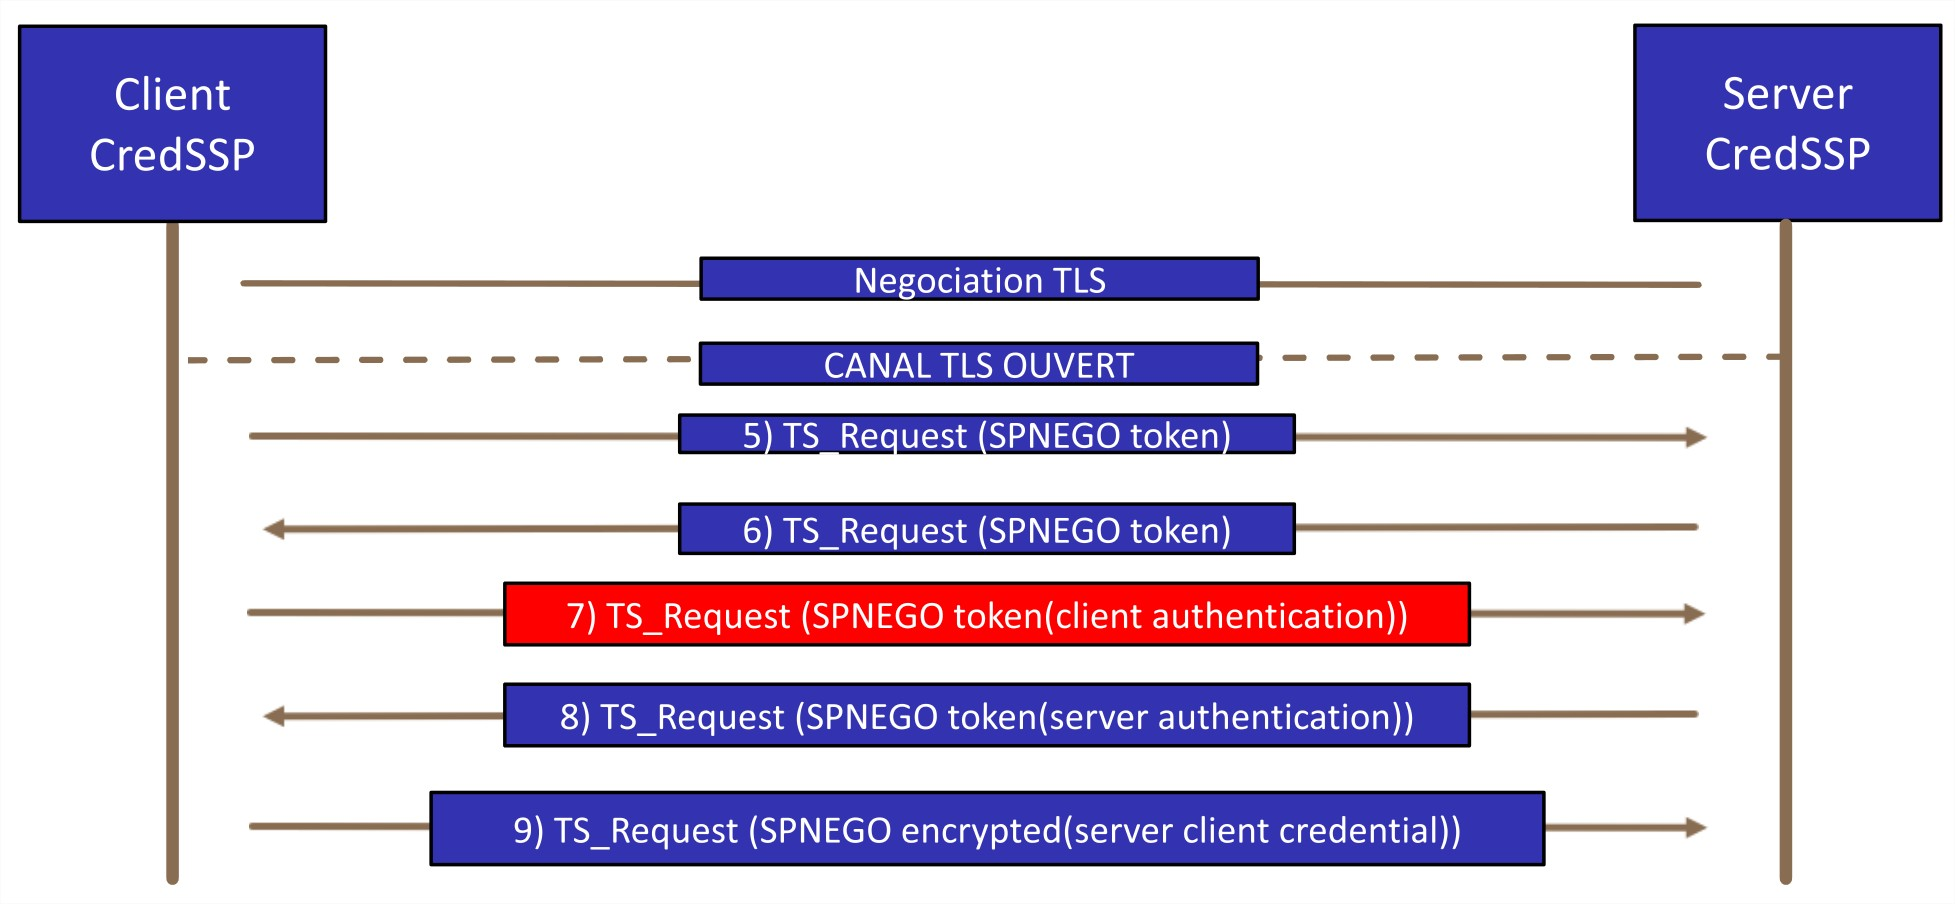
\includegraphics[scale=0.07]{step7.jpg}
	 \end{columns}
	 
	 \begin{itemize}
	 	\item NTLMSSP AUTHENTICATE\_MESSAGE est la réponse au challenge contenant :
	 		\begin{itemize}
	 		\item NTLMv2 response
	 		\item Username
	 		\item Domain name
	 		\item EncryptedSessionKey = $\underset{NTLMKey}{RC4}$(RandomSessionKey) - NTLMKey : HMACMD5 derivé du NTLM Challenge et creds
	 		\end{itemize}
	 	\end{itemize}
\end{frame}

%slide 10
\begin{frame}[fragile]{CredSSP - NTLMSSP Etape 7}
	 \begin{columns}[T]
	 \column{0.7\textwidth}
	 	\begin{itemize}
	 	\item Le client répond au challenge et demande une vérification de l'intégrité de l'échange TLS
	 	\end{itemize}
	 \begin{lstlisting}[frame=single,basicstyle=\tiny]
TSRequest {
	Version:     6,
	negoToken:   NegoData-> NTLMSSP AUTHENTICATE\_MESSAGE,
	pubKeyAuth: Signature + encryptedpubKey,
	clientNonce: Octet String
	}
	\end{lstlisting}
	 \column {0.3\textwidth}
	 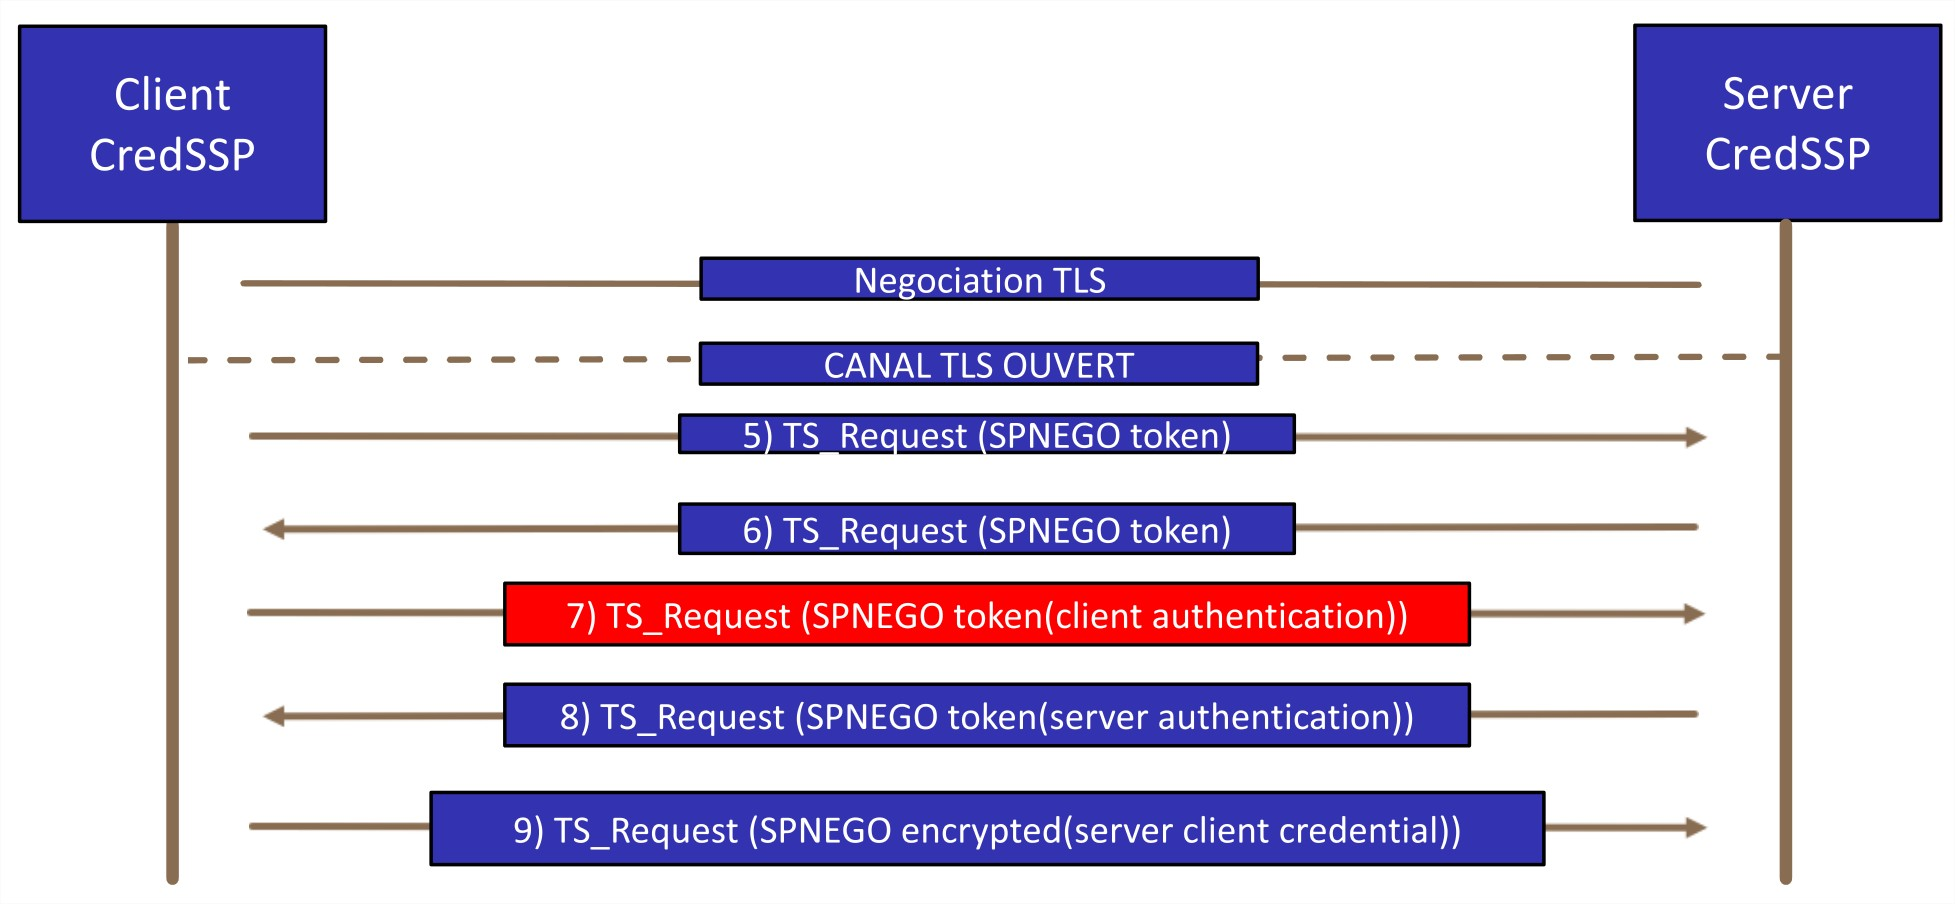
\includegraphics[scale=0.07]{step7.jpg}
	 \end{columns}
	 
	 \begin{itemize}
	 	\item pubKeyAuth contient :
	 		\begin{itemize}
	 		\item $\underset{RandomSessionKey}{RC4}$(SHA256('CredSSP Client-To-Server Binding Hash' + Nonce + PublicKey))
	 		\end{itemize}
	 	\end{itemize}
	 	
Le serveur peut alors vérifier l'intégrité de la connexion TLS en vérifiant le champs pubKeyAuth.
Pour cela il a besoin de la valeur de RandomSessionKey (envoyée par le client mais chiffrée à l'aide de la NTLMKey)
\end{frame}

%slide 11
\begin{frame}[fragile]{CredSSP - NTLMSSP Etape 7 (vérification serveur)}
	 \begin{columns}[T]
	 \column{0.7\textwidth}
	 	\begin{itemize}
	 	\item Si le compte appartient au domaine :
	 		\begin{itemize}
	 		\item Le serveur s'authentifie auprès du DC via DCE-RPC
	 		\item Le serveur transmet la réponse NTLMv2 auprès du DC (NetLogonSamLogonwithFlags request)
	 		\item Le DC authentifie le client et envoie au serveur la NTLMKey
	 		\item Le serveur déchiffre alors encryptedSessionKey et récupère la RandomSessionKey
	 		\item Le serveur déchiffre PubKeyAuth et vérifie l'intégrité du canal TLS
	 		\end{itemize}
	 	\end{itemize}
	 \column {0.3\textwidth}
	 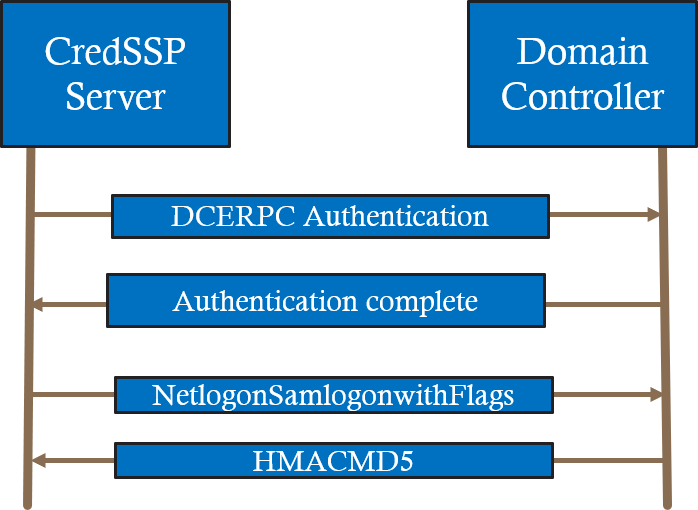
\includegraphics[scale=0.3]{graph2.png}
	 \end{columns}
\end{frame}

%slide 12
\begin{frame}[fragile]{CredSSP - NTLMSSP Etape 8 }
	 \begin{columns}[T]
	 \column{0.7\textwidth}
	 	 \begin{lstlisting}[frame=single,basicstyle=\tiny]
TSRequest {
	Version:     6,
	pubKeyAuth: Signature + encryptedCertificate,
	}
	\end{lstlisting}
	 \column {0.3\textwidth}
	 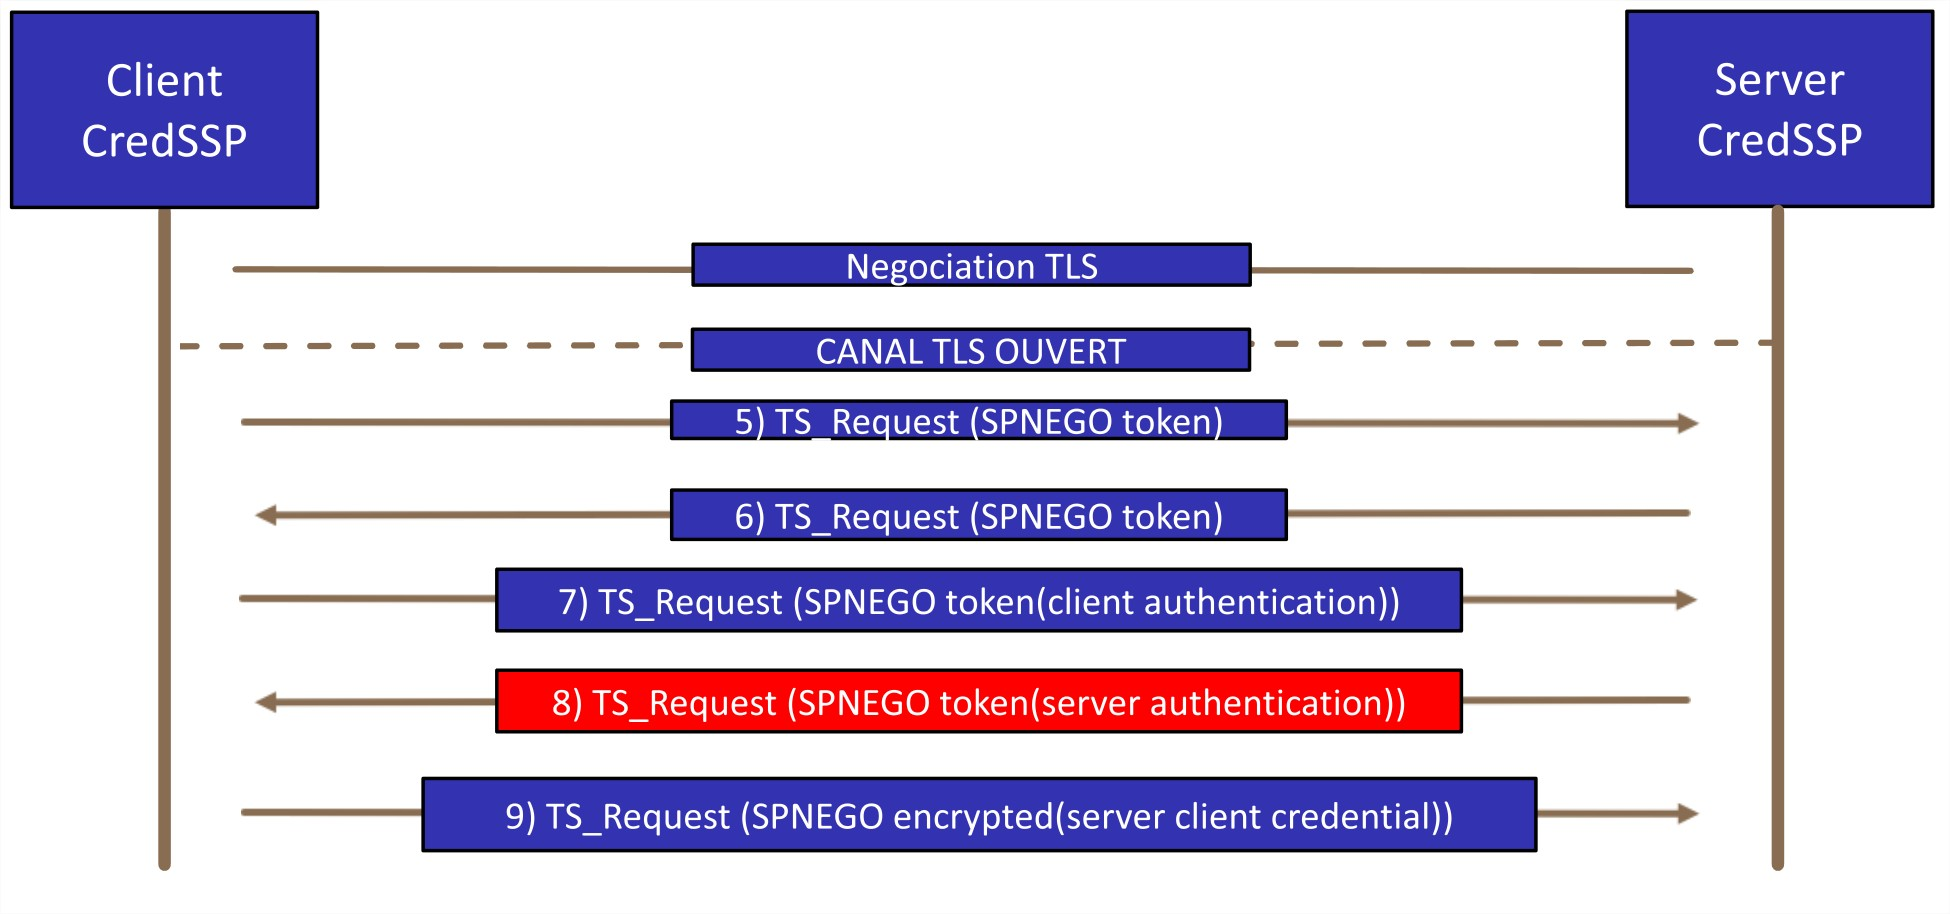
\includegraphics[scale=0.07]{step8.jpg}
	 \end{columns}
	 	 	\begin{itemize}
	 	\item pubKeyAuth contient:
	 		\begin{itemize}
	 		\item $\underset{RandomSessionKey}{RC4}$(SHA256('CredSSP Server-To-Client Binding Hash' + Nonce + PublicKey))
	 		\item Les différences sur les versions de CredSSP sont notables sur la manière de chiffrer ces informations \newline
	 		
			\end{itemize}
			\item \textbf{Conclusion: } « L'authentification mutuelle » permet seulement de vérifier que le serveur peut récupérer la NTLMKey i.e. qu'il est en mesure de s'authentifier auprès du DC
	 	\end{itemize}
\end{frame}

%slide 13
\begin{frame}[fragile]{CredSSP - NTLMSSP Step 8 }
Le client va-t'il envoyer ses authentifiants maintenant? 
\begin{itemize}
\item Non, cette vulnérabilité a été patchée dans RDP 7.0\newline

\end{itemize}
L'ensemble du process va recommencer une deuxième fois et montrer le certificat à l'utilisateur\newline

Cependant l'attaquant en position de singe intercepteur aura déjà obtenu une réponse NTLMv2 valide (en vue d'un cassage ou d'un relai) 
\end{frame}


%slide 15
\begin{frame}[fragile]{CredSSP - NTLMSSP Etape 9 }
Dans le cas ou le client accepte le certificat, l'échange recommence et va jusque l'étape 9 \newline
\begin{center}
 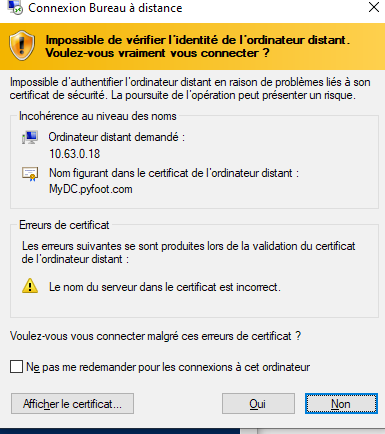
\includegraphics[scale=0.31]{Cert.png}
 \end{center}
 \textbf{N.B. :} L'utilisation de l'adresse IP par le client pour la connexion auprès du serveur, générera dans le cas général une erreur de certificat
\end{frame}

%slide 16
\begin{frame}[fragile]{CredSSP - NTLMSSP Etape 9 }
	 \begin{columns}[T]
	 \column{0.7\textwidth}
	 	 \begin{lstlisting}[frame=single,basicstyle=\tiny]
TSRequest {
	Version:     6,
	authInfo: Signature + cryptedCreds,
	}
	\end{lstlisting}
	\column{0.3\textwidth}
	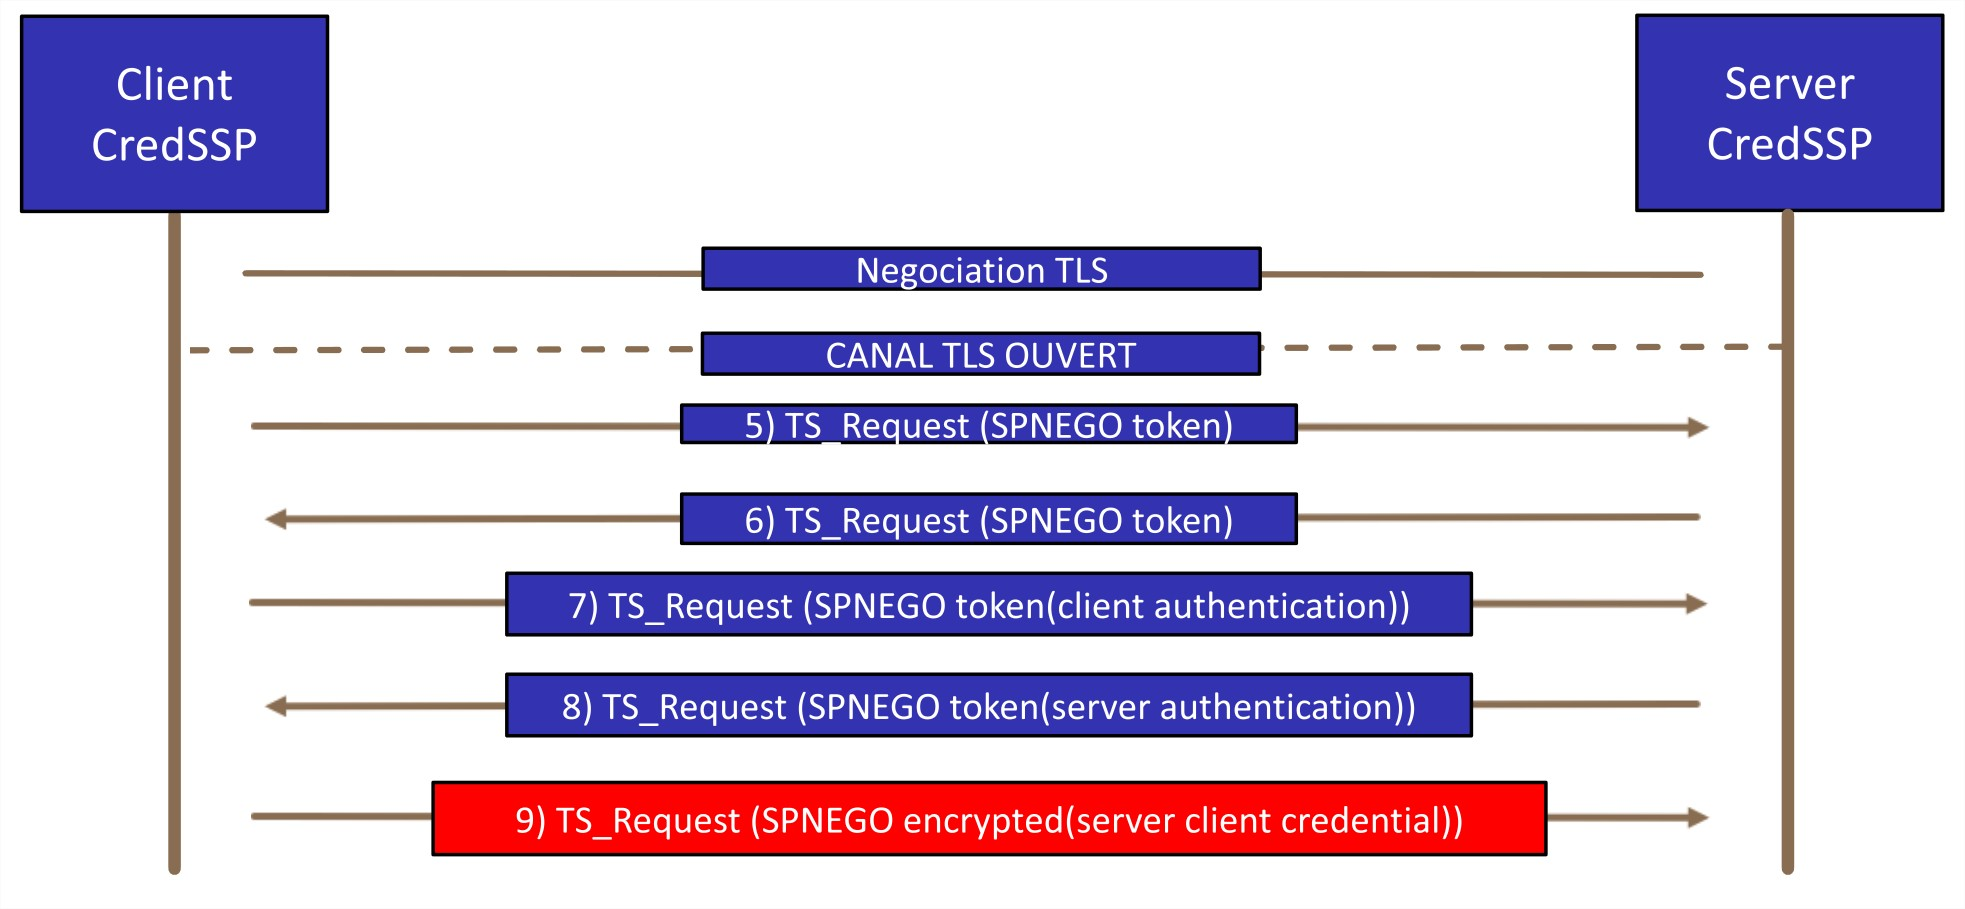
\includegraphics[scale=0.07]{step9.jpg}
	\end{columns}
		\begin{itemize}
		\item AuthInfo contient:
			\begin{itemize}
			\item $\underset{RandomSessionKey}{RC4}$(Credentials Structure)
			\end{itemize}
		\item Credentials Structure contient le mode d'authentification (password, smartcard,...) et les authentifiants
		\end{itemize}
\end{frame}

%slide 17
\begin{frame}[fragile]{CredSSP - Demo}
	 \begin{center} DEMO
	 \end{center}
\end{frame}

\section{Kerberos Downgrade}

\begin{frame}
	\frametitle{Table des matières}
	\tableofcontents[currentsection]
\end{frame}
%slide 18
\begin{frame}[fragile]{CredSSP - Kerberos}
Quelles sont les différences?
\begin{itemize}
\item Le NegoData contient maintenant un TGS valide à destination du serveur contenant la randomSessionKey
\item De fait il n'est plus possible d'utiliser n'importe quel compte machine pour réaliser l'attaque
\item Cependant, il est possible de partiellement downgrader cette connexion
\end{itemize}
\end{frame}

%slide 19
\begin{frame}[fragile]{CredSSP - Kerberos Etape 5}
Lors de la négociation du SSP, la TSRequest du client est de cette forme:
\begin{lstlisting}[frame=single,basicstyle=\tiny]
TSRequest {
	Version:     6,
	NegoToken: Kerberos,
	}
	\end{lstlisting}
	
Même si le client supporte NTLMSSP, il n'est pas proposé par le client
\end{frame}

%slide 20
\begin{frame}[fragile]{CredSSP - Kerberos Etape 6}
Cependant il est possible de forcer le client à utiliser NTLMSSP en envoyant un paquet SPNEGO\_RENOGOCIATE
\begin{lstlisting}[frame=single,basicstyle=\tiny]
TSRequest {
	Version:     6,
	NegoToken: \xa1\x...NTLMSSP\x00\x00...\x0f,
	}
	\end{lstlisting}
À réception de ce message, le client accepte maintenant d'utiliser NTLMSSP mais... le protocole CREDSSP est maintenant complétement « cassé »
\end{frame}

%slide 20.5
\begin{frame}[fragile]{CredSSP - Kerberos Etape 6}
Pour des raisons inconnues, le message NTLM NEGOTIATE\_MESSAGE est maintenant dans le champ AuthInfo dans une TSRequest encapsulée dans le champ « NegoData »
\begin{lstlisting}[frame=single,basicstyle=\tiny]
TSRequest {
	Version:     6,
	NegoToken: TSRequest{
		Version: 1
		AuthInfo : NTLMSSP NEGOCIATE\_MESSAGE
		}
	}
	\end{lstlisting}

\end{frame}

%slide 21
\begin{frame}[fragile]{CredSSP - Kerberos Step 6}
Il suffit maintenant de répondre avec un challenge NTLMv2 et d'utiliser la même structure pour l'envoi des informations :


\begin{lstlisting}[frame=single,basicstyle=\tiny]
TSRequest {
	Version:     6,
	NegoToken: TSRequest{
		Version: 1
		AuthInfo : NTLMSSP CHALLENGE\_MESSAGE
		}
	}
	\end{lstlisting}

\end{frame}

%slide 22
\begin{frame}[fragile]{CredSSP - Kerberos Step 7}
Le client répondra avec sa réponse NTLMv2 suivant la même structure
\begin{columns}[T]
\column{0.7\textwidth}
\begin{lstlisting}[frame=single,basicstyle=\tiny]
TSRequest {
	Version:     6,
	NegoToken: TSRequest{
		Version: 1
		AuthInfo : NTLMSSP AUTHENTICATE\_MESSAGE
		},
	pubKeyAuth : NULL
	ClientNonce : NULL
	}
	\end{lstlisting}
\column{0.3\textwidth} 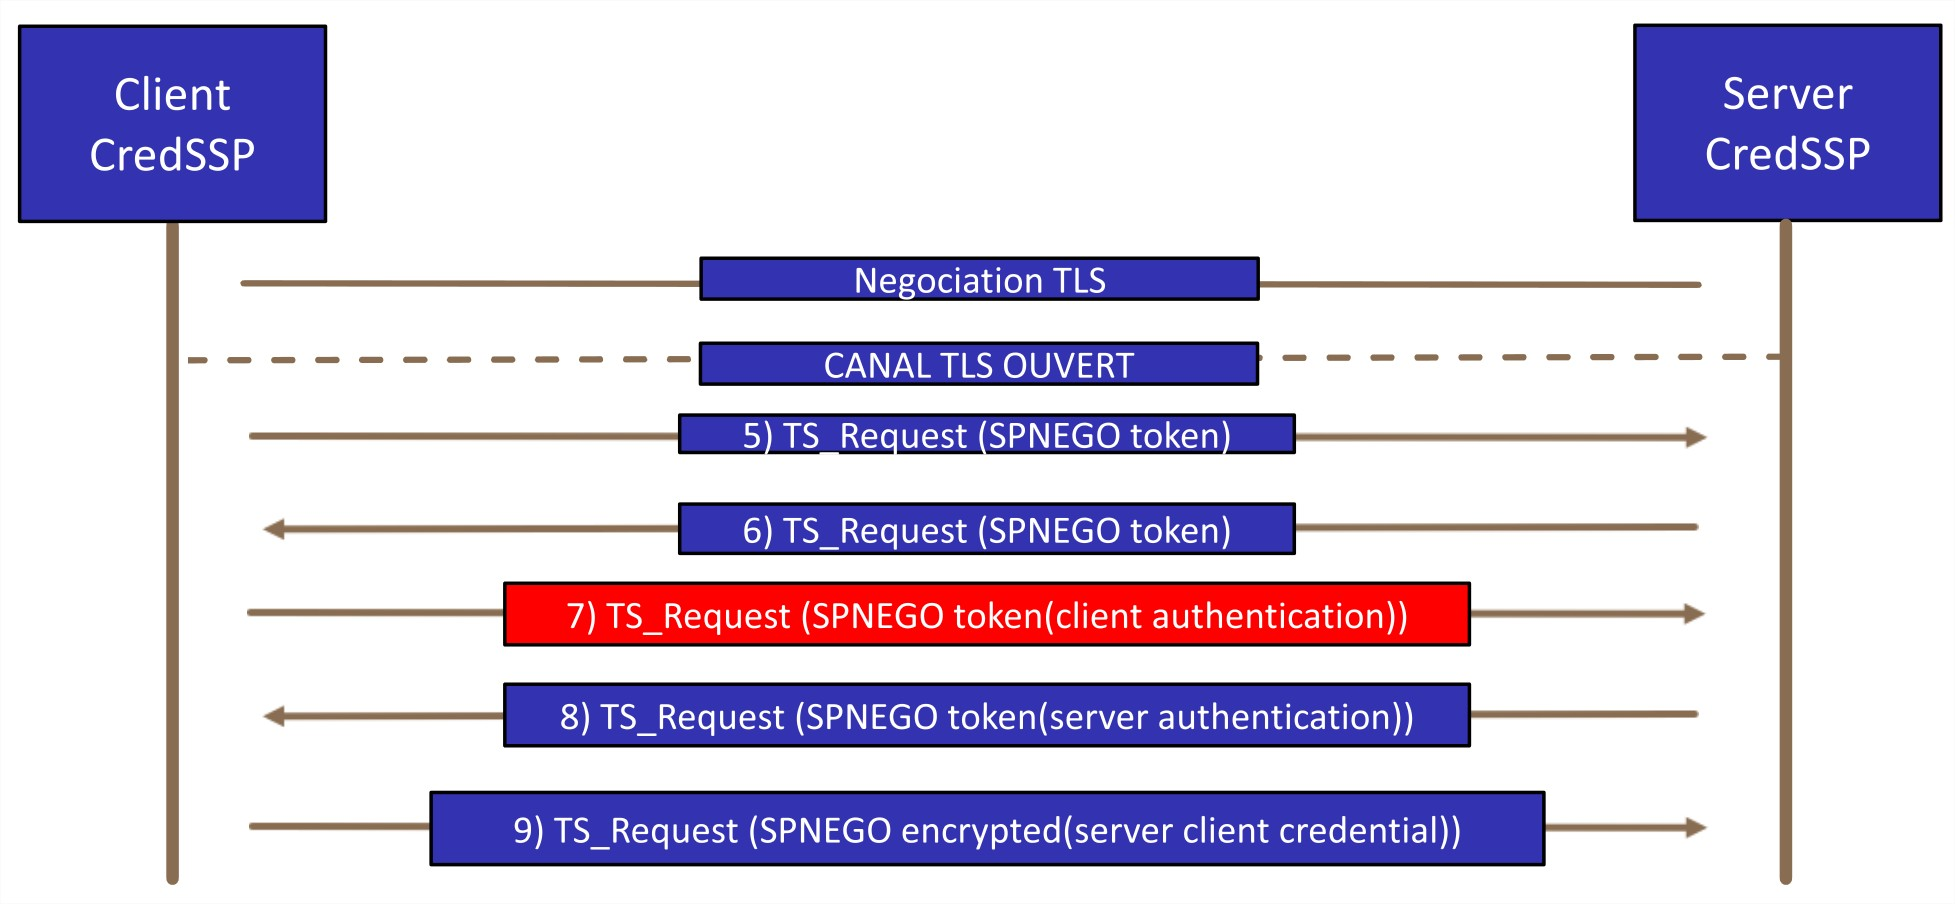
\includegraphics[scale=0.07]{step7.jpg}
\end{columns}
Cependant il n'envoie aucune information Cryptographique (RandomSessionKey, etc.), il n'est donc pas possible de répondre de manière valide auprès du client

\textbf{La connexion va alors échouer mais l'attaquant a obtenu une réponse NTLMv2 valide sans générer d'alerte sur le certificat de la connexion}
\end{frame}

%slide 23
\begin{frame}[fragile]{CredSSP - Downgrading Kerberos Auth}
	 \begin{center} DEMO
	 \end{center}
\end{frame}


%slide 22
\begin{frame}[fragile]{CredSSP -- Kerberos Bonus}
\begin{itemize}
\item Protected Users ajoute des protections sur la gestion de l'authentification :
	\begin{itemize}
	\item Empêche de se loguer via NTLM
	\item Empêche le cache d'authentifiants
	\item Empêche l'utilisation de RC4 (NTLM) pour la pré-authentification Kerberos
	\end{itemize}
	\item À titre d'exemple, lorsqu'un Protected User utilise une adresse IP pour se connecter à un partage réseau, aucune requête NTLMSSP n'est envoyée
\end{itemize}
\textbf{Il est tout de même possible de récupérer une réponse NTLMv2 d'un utilisateur Protected User, il ne sera pas contre pas possible de faire du relai avec}
\end{frame}

%slide 22
\begin{frame}[fragile]{CredSSPY }
\begin{itemize}
\item L'outil ne fonctionne actuellement que contre le client officiel Microsoft :
	\begin{itemize}
	\item Le client Mac Microsoft et FreeRDP vérifie le certificat à la première connexion
	\item Le client Mac Microsoft et FreeRDP ne comprennent pas le paquet permettant le downgrade Kerberos
	\end{itemize}
\item L'outil est toujours en Beta, des évolutions pourrait être:
	\begin{itemize}
	\item Ajouter les fonctionnalités d'authentification NLA dans rdpy ou PyRDP afin de profiter des fonctions d'enregistrements de sessions ou de capture des frappes claviers
	\item Implémenter le RelayNTLMSSP
	\end{itemize}
\end{itemize}
\end{frame}


%slide 24
\begin{frame}[fragile]{Questions}
	 \begin{center}	 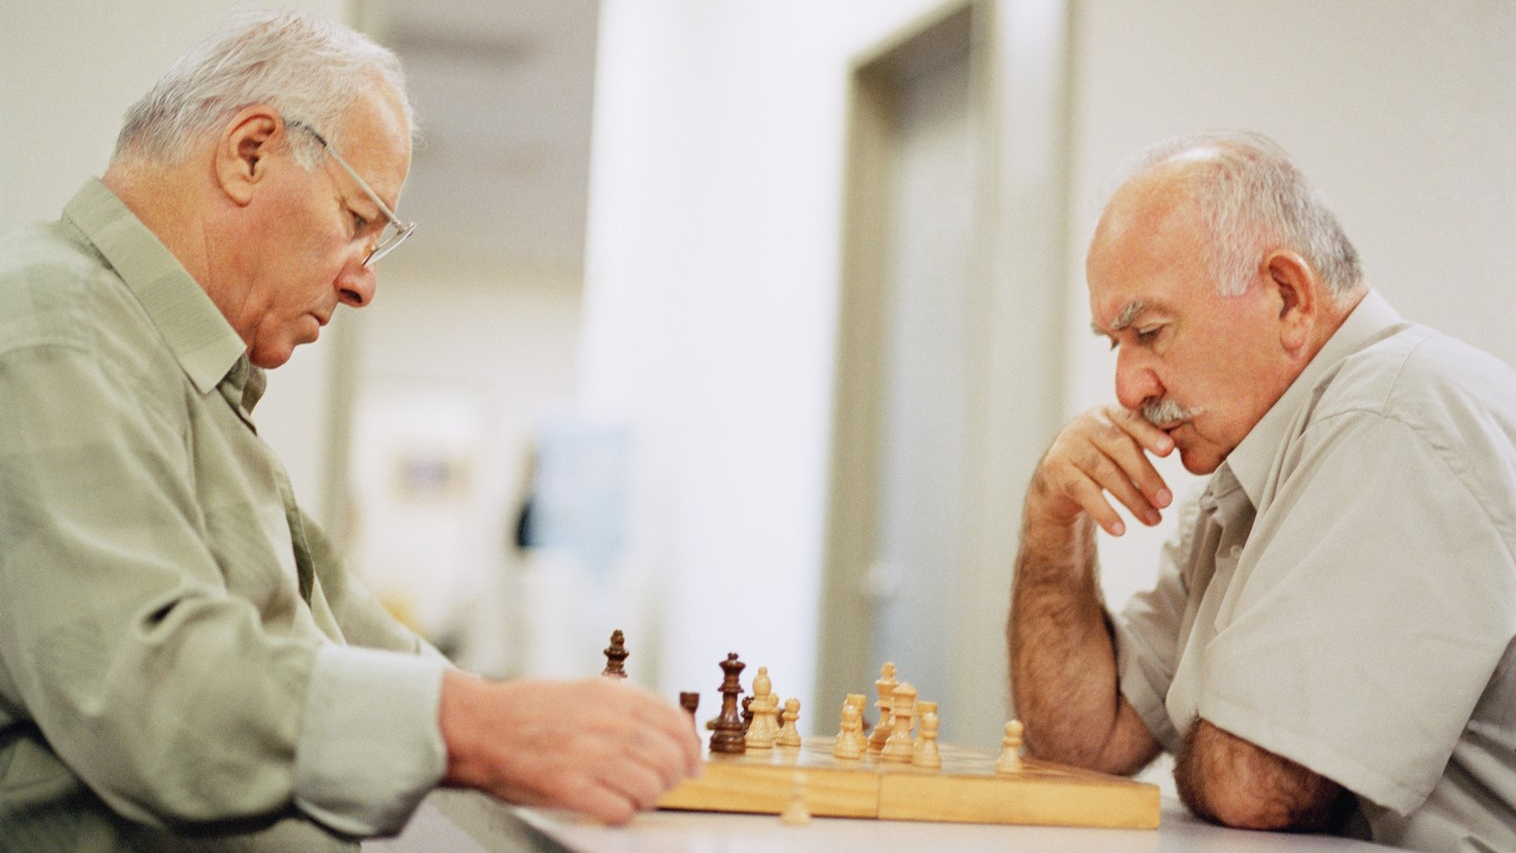
\includegraphics[scale=0.26]{vieux.png}
	 \end{center}

\end{frame}
\end{document}
